\section[REVISÃO DA LITERATURA]{revisão da literatura}

A pesquisa da base bibliográfica utilizada neste trabalho considerou a busca por livros,
teses, monografias e artigos nas seguintes fontes especializadas: PubMed, ACM
(Association for Computing Machinery), IEEE (Institute of Electrical and Electronics
Engineers), RadiologySource, Radiographics, USP (Universidade de São Paulo), UFSC
(Universidade Federal de Santa Catarina) e IBICT (Instituto Brasileiro de Informações em
Ciência e Tecnologia).

O PubMed é uma base de dados que permite a pesquisa bibliográfica de artigos
publicados em revistas de grande circulação da área médica. Ele foi desenvolvido pelo
NCBI (National Center for Biotechnology Information), sendo mantido pela NLM
(National Library of Medicine). A pesquisa realizada com a palavra-chave “FFDM”
retornou 112 trabalhos, dos quais apenas dois foram relevantes ao tema em estudo. Nessa
mesma base, uma pesquisa com o argumento “digital mammography integration” implicou
em 27 trabalhos, dos quais apenas dois foram de real interesse. O cruzamento dos dados
das duas pesquisas resultou em dois trabalhos de interesse.

Os mesmos parâmetros de pesquisa foram aplicados na base ACM, resultando em 17
trabalhos para a palavra-chave “FFDM” e nenhum trabalho para “digital mammography
integration”. Analisando os 17 trabalhos resultantes da primeira pesquisa, constatou-se que
nenhum deles tratou dos procedimentos para a execução de projetos de integração com
mamógrafos digitais.

Outra base bibliográfica pesquisada foi o IEEE. Embora a pesquisa tenha retornado
seis trabalhos para a palavra-chave “FFDM” e sete trabalhos para “digital mammography
integration”, nenhum deles versou sobre o tema abordado neste trabalho.

A base de dados denominada de RadiologySource foi a que melhor apresentou
resultados de trabalhos associados ao tema em estudo. A pesquisa pela palavra-chave
“digital mammography integration” retornou 15 trabalhos, dos quais seis foram de
relevância para o assunto estudado. A RadiologySource é uma base bibliográfica que
publica artigos da área de radiologia oriundos de revistas de prestígio, algumas delas
acreditadas pelo ACR (American College of Radiology).

Outra base de dados utilizada na pesquisa bibliográfica foi a Radiographics, uma
revista com tiragem bimestral que tem como objetivo, promover a educação continuada na
área da radiologia. A pesquisa pela palavra-chave “digital mammography integration”
retornou seis trabalhos, dos quais três foram importantes para o objeto desta pesquisa.

No Brasil, foram consultadas as bases bibliográficas da USP, UFSC e do IBICT.
Apenas a base do IBICT retornou dois resultados ao se utilizar as palavras-chaves
“integração” e “mamografia digital”. Entretanto, nenhum dos trabalhos encontrados é de
relevância ao tema tratado neste documento.

Devido à grande variedade de assuntos associados ao objeto de estudo, foram
realizadas outras pesquisas nas bases de dados citadas, de modo a identificar trabalhos nas
seguintes áreas de conhecimento: Mamografia Digital, DICOM (Digital Imaging
Communications in Medicine), IHE (Integrating the Healthcare Enterprise), RIS e PACS.
O resultado dessas pesquisas isoladas foi muito promissor e é resumido na descrição a
seguir, que sumariza o rol de trabalhos relevantes para esta pesquisa.\\
...

...
A Figura \ref{esquematico} mostra, respectivamente, um diagrama esquemático de um equipamento de
mamografia e um desenho ilustrativo de um mamógrafo.

\begin{figure}[ht]
 \centering
 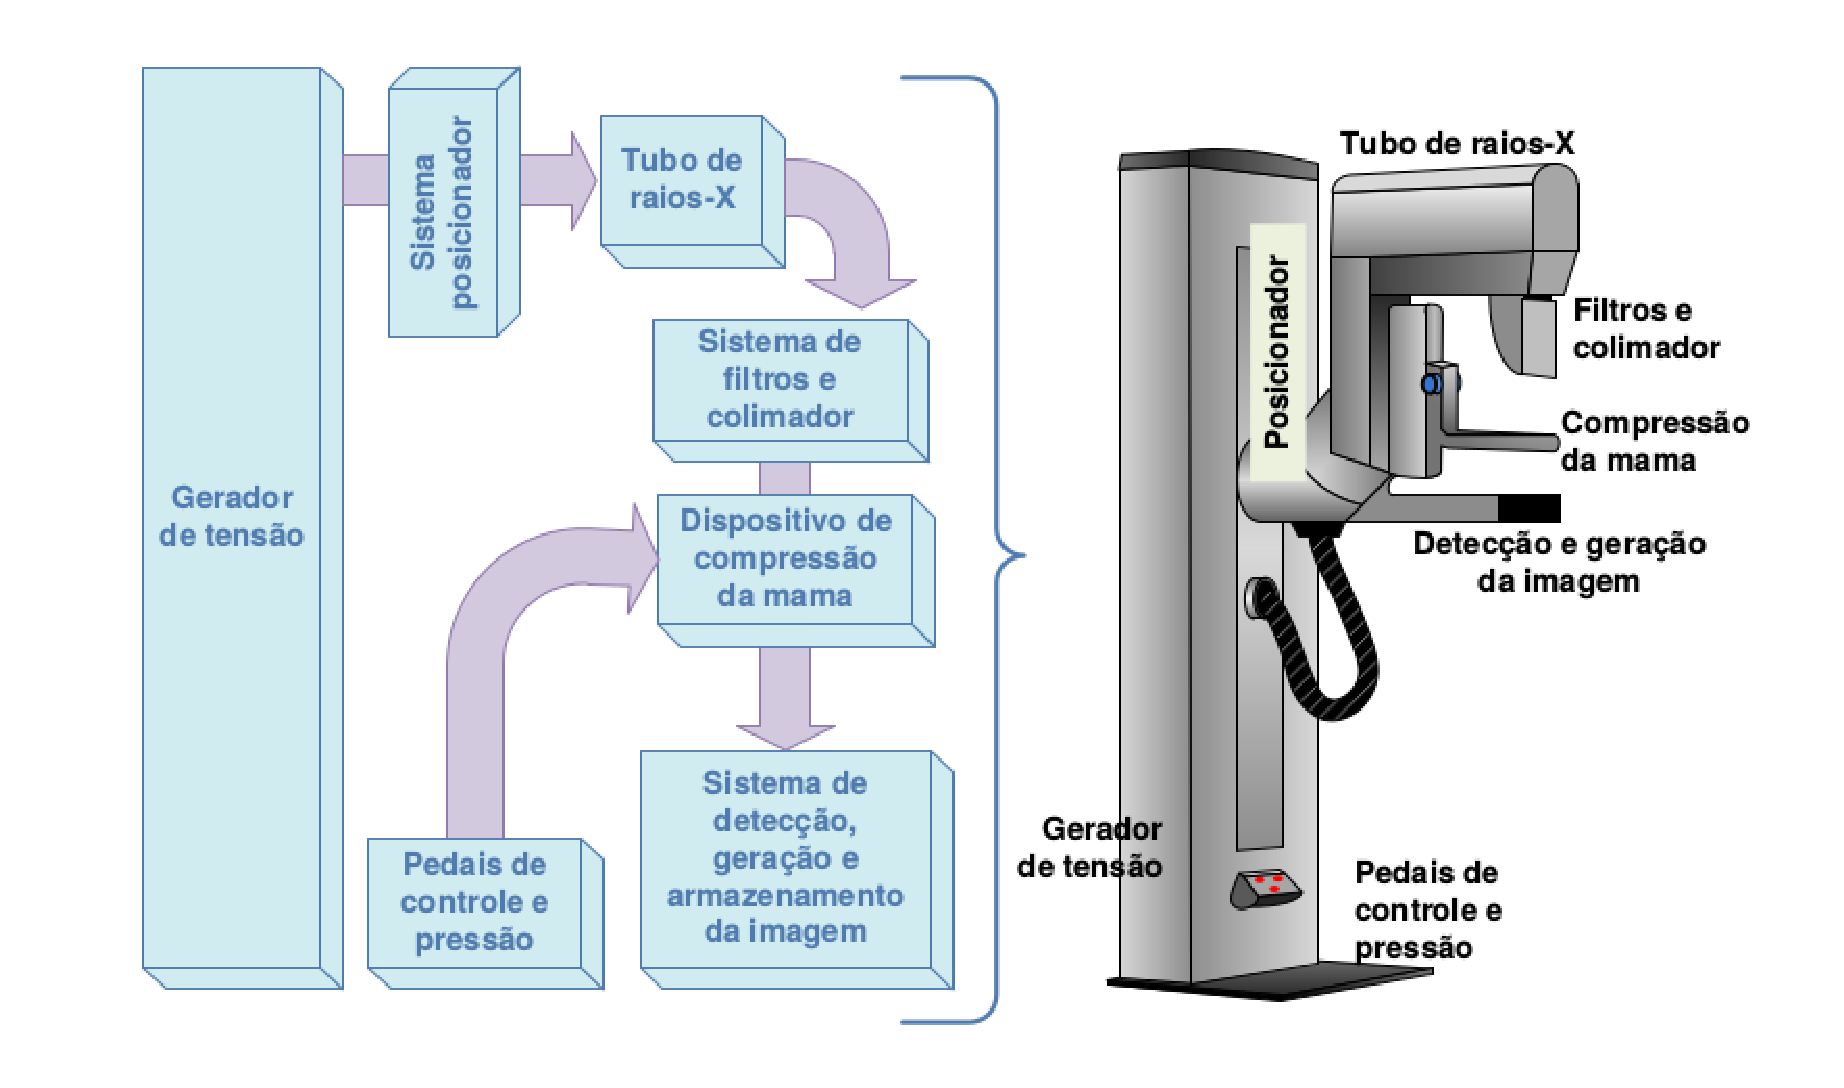
\includegraphics[width=15 cm]{figuras/fig1.eps}
 \caption{Esquemático do mamógrafo (Modificado de MINISTÉRIO DA SAÚDE, 2002).}
 \label{esquematico}
\end{figure}





